\section{Physical Operators and Implementation}

For each of the logical operators there are different physical implementations.
We do not currently select the appropriate physical operator and the user has to specify this.
We do, however, set sensible default parameters for each of the physical operators.
In \projx, there are three broad categories of physical operators: Automated, Crowd, and Learning.
An automated physical operator is conceptually the same as a SQL user defined function, while a crowd operator uses a microtask platform.
A learning operator takes in training examples (whether crowd or ground truth) and learns an automated operator.
We describe each below.

\ewu{below are straightforward physical implementations of the
logical operators.  Is there anything interesting to say about their
design or a specific physical operator?}

\team{How do we know when transitive closure/any of the physical operators can be safely applied?  Are there properties of the physical ops that could tell us?}


\subsection{Similarity Join} 
\projx provides a library of the following commonly used similarity functions: \textsf{JaccardSimilarity}, \textsf{DiceSimilarity},
\textsf{CosineSimilarity}, \textsf{OverlapSimilarity}, and \textsf{EditDistance}.
The user can select one of these similarity functions.
A naive implementation of a Similarity Join is to take the cartesian product and then filter all pairs of record of similarity greater than $t$.
However, the implemented similarity functions are all symmetric and the similarity function is maximized when $r = p$.
So it suffices to compute a similarity $\theta$-join instead of the full Cartesian product.
We can further add an optimization called prefix filtering to further reduce the number of similarity function evaluations.
In prefix filtering, we prune pairs that cannot possibly meet the threshold $t$ based on the number of tokens that overlap which can be determined with an inverted index.


\subsection{Extraction}
We implement basic automated extraction libraries including delimited splitting and regular expression methods.
However, extraction is a task that is well suited for crowd sourcing.
We provide a parametrized interface that allows the user to specify an extraction attribute, a formatting question, and request data from the crowd.
In Figure \ref{fig:entry}, we illustrate an example of this task.

\begin{figure}[ht!]
\centering

\includegraphics[scale=0.25]{figs/entry.png}
\caption{Example of the Extraction Crowd Interface. \label{fig:entry}}\vspace{-.5em}
\end{figure}

\subsection{Filtering}
We provide an interface for a user defined predicate.
However, as with extraction, filtering has many opportunities for crowdsourcing.
For a filtering operation, the crowd response is binary in contrast to Extraction.
We provide crowd templates for two types of filtering tasks.

\noindent\textbf{Condition Checking: } Given a single record, a crowd worker indicates if it satisfies some condition. In Figure \ref{fig:condition},
we illustrate an example condition checking task.
\begin{figure}[ht!]
\centering
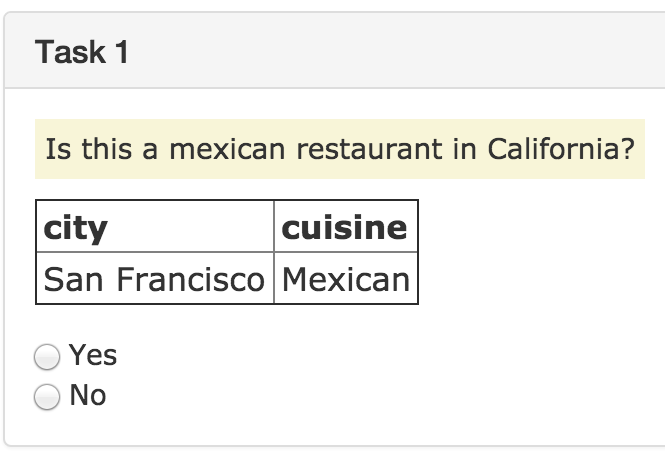
\includegraphics[scale=0.25]{figs/condition.png}
\caption{Condition checking is one variant of the filtering crowd interface.\label{fig:condition}}\vspace{-.5em}
\end{figure}

\noindent\textbf{Pair Comparison: } Given a pair of records, a crowd worker indicates if they are the same or are different. In Figure \ref{fig:pair},
we illustrate an example pair comparison task.

\begin{figure}[ht!]
\centering
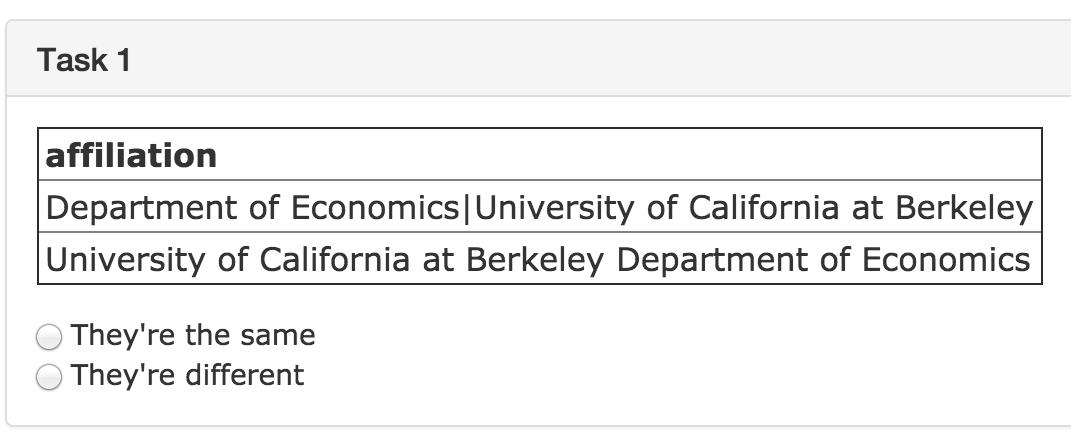
\includegraphics[scale=0.25]{figs/pair.png}
\caption{Pair comparison is the other variant of the filtering crowd interface.\label{fig:pair}}\vspace{-.5em}
\end{figure}



\subsection{Extended Operators}

\subsubsection{Sampling}
\projx provides different variants of uniform sampling.
We provide Bernoulli sampling (in which flips a ``biased coin" for each row) or hash sampling (which hashes an attribute).
Hash sampling allows for joining sampled relations with foreign key relationships.
On the other hand, Bernoulli sampling is less sensitive to skews and leads to more consistent sample sizes.

\subsubsection{Transitive Closure}
Similarity Joins can create issues with transitivity.
For example, rowA might be similar to rowB and rowB might be similar to rowC, but rowA might not be similar to rowC.
We can associate these relationships with edges in a similarity graph.
Then to enforce transitive closure, we solve a connected components problem.
We apply a distributed using a distributed gather-apply-scatter connected components algorithm in the Spark-integrated graph library GraphX.



